
\chapter{Introduction}
\label{ch:introduction}

This chapter introduces the project's motivation, its objectives, the methodology followed, the problem that we are tackling and the experimental set up. 

This thesis is structured as follow. %First an introduction to the problem we want to solve is presented in Chapter \ref{ch:introduction}. Then, iThis work is structured as follow. First an introduction to the problem we want to solve is presented in Chapter \ref{ch:introduction}. 
In Chapter \ref{ch:state_of_the_art} a review of the current state of the art in manipulation planning is done. The planning system developed and the algorithm to generate the states will be explained in Chapters \ref{ch:planning_system} and \ref{ch:implementation} respectively. In Chapter \ref{ch:software_design} the software design will be presented as well the algorithm's structure. Finally  experiments and conclusions about this work are discussed in Chapters \ref{ch:experiments} and \ref{ch:conclusions} respectively.n Chapter \ref{ch:state_of_the_art} a review of the current state of the art in manipulation planning is done. The planning system developed and the algorithm to generate the states will be explained in Chapters \ref{ch:planning_system} and \ref{ch:implementation} respectively. In Chapter \ref{ch:software_design} the software design will be presented as well the algorithm's structure. Finally  experiments and conclusions about this work are discussed in Chapters \ref{ch:experiments} and \ref{ch:conclusions} respectively.

\section{Project motivation}
Robotic manipulation of objects is an increasing field of research which has captured the interest of researches from many years ago. In several industrial environments robots can be easily programmed when the objects are known a priori, i.e. the manipulation is always the same, and robot operations avoid cluttered scenes, but the workspace has to be designed in a manner to provide to the robot a non cluttered scene. However, there are situations in which robots with enhanced intelligence can be useful.
 An example in which a robot could face a cluttered scenario is the one of the \textit{Amazon Picking Challenge} \citep{APC}, which provides a challenge problem to the robotics research community that involves integrating the state of the art in object perception, motion planning, grasp planning, and task planning to manipulate real-world items in industrial settings such the ones human operators face in Amazon's warehouse. Joey Durham from Amazon Robotics describes the challenges of this competition as follows:
\begin{displayquote}
 “A robot for picking purposes must possess a lot of skills: The selected item must be identified, handled and deposited correctly and safely. This requires a certain level of visual, tactile and haptic perceptive skills and great handling capabilities.”
\end{displayquote}

In this thesis we investigate a simple approach for a complex manipulation problem. Our approach tries to replicate human reasoning during the manipulation of cluttered objects in table clearing tasks. The objective is removing all the objects on a table. 

This master thesis has been developed in the \textbf{Institut de Robòtica i Informàtica Industrial} (IRI) in the  Perception and Manipulation laboratory with the supervision of \textit{Guillem Alenyà Ribas} as director and \textit{David Martínez Martínez} as co-director. 






%\section{Project motivation}
%\todo[inline]{merge with the previous paragraph}
%This project is motivated by the increasing interest by the scientific community regarding the artificial intelligence for robots. Robotic manipulators are widely used in industry, to solve standard tasks which can be solved programatically by algorithms, such as a soldering robotic manipulator. 
%But there are cases in which an enhanced intelligence for the robot could be useful. These manipulators have the goal to substitute humans in repetitive tasks such the one to clean an table of objects, or to grasp a specific object in complex scenes. The latter is the case of the \textit{Amazon Picking Challenge}.  
%The manipulation of objects is an important area of research with an advanced state of the art regarding grasping objects. But still there is a gap to make them completely autonomous to resolve manipulation problem. The robots not always can grasp an object because adjacent objects hinder that action, so the robot needs to interact with the objects in a intelligent way in order to achieve the goal. In this thesis we investigate a intelligence system which can reasons about how to interact with the objects in order to achieve the goal to grasp an object, or grasp them all. 

%With these considerations we think the thesis is well motivated since the work is focused in an important area of research in robotics. 

\section{Objectives}
The objective of this thesis is designing and implementing an artificial intelligence system which can reason about how to interact with the objects in order to clear a table with cluttered objects. To clear a table means grasp all the objects and removed them by dropping them, for example, in a bin. To do so a robotic manipulator is used in order to interact with the objects. The idea is to design the planning system by human-inspired actions, that is the intelligence system we want to develop tries to solve the task similarly as a human would do.

\section{Methodology}
The methodology we will follow for the project is composed of 5 phases:
\begin{enumerate}
\item documentation,
\item designing of the algorithm,
\item implementation,
\item tests in simulations and with the real robot,
\item analysis of the results. 
\end{enumerate}
The documentation regards reviewing the state of the art in manipulation planning and gathering all the others information required to design properly the algorithm such as objects segmentation, plane detection, grasping and etcetera. Next the algorithm will be designed and then implemented. After the implementation it will be tested in a simulated environment (Chapter \ref{ch:software_design}) and then 
with the real set up (Chapter \ref{ch:experiments}). Then the results will be analysed in order to have some conclusions about the proposed planning system. 

\section{Problem Approach}
In this section the approach to solve the planning problem is described. The strategy to solve the problem is inspired by the way humans solve it. A human would use mainly two actions: grasping and pushing. When it is not possible to grasp an object, because other objects hinder the human to put the hands in the proper way to grasp the desired one, he/she interacts with the scene to make the object graspable. However,  humans are characterized by a high dexterity and therefore they have a lot of freedom in the way to grasp objects. Robots, normally, do not have such a dexterity and grasping in cluttered scene could be very hard without moving the objects. 

The pushing action requires to put the end effector in a certain pose and then push the object by moving the end effector. However, it is difficult to push an object and ensure that it follows the desired path since this action depends on its shape. Moreover a controller would be needed in order to correct the pose of the end effector along the path. We assumed that all objects had basic shapes, so that a simple pushing action performs well.

Based on these considerations, the actions the robot has to use are grasping and pushing.
Grasping is the most important action since it lets to take an object and drop it somewhere, for instance into a bin, clearing in this way the table. There exist different works facing the same task by focusing only in grasping \citep{haf,AGILE}. The pushing is useful when two adjacent objects could not be grasped if they are so close such that the robot's gripper, when attempting to grasp an object, is going to collide with the adjacent one, making the object ungraspable. The pushing action can separate adjacent objects that mutually exclude themselves from being grasped. 
For simplicity we only consider actions that interact with a single object.% \DMcomment{For example, humans may push several objects together in some cases...}

The robot's decision maker uses a planning system that returns a sequence of actions that achieve the goal of clearing the table. 
The robot reasons in an abstraction level by considering only symbolic predicates with limited geometrical information. Then the plan is checked to see if it is feasible, and if it isn't, backtracking is done.
%The robot reasons in an abstraction level by considering only symbolic predicates which are obtained by hand-built mapping functions making the reasoning step simpler. It is important noting that this problem should includes relevant geometric information which are very useful for the planner, such as how much to push an object, in what direction and the inverse kinematic of the robot. This geometric information is translated into symbolic literals, although these are not able to catch all the geometric information. Then the plan is checked to see if it is feasible, and if it isn't, backtracking is done. \DMcomment{This paragraph is too complicated. Just say that the robot reasons in a symbolic level (planning) with limited geometrical information. Then the plan is checked to see if it is feasible, and if it isn't, backtracking is done.}

We assume the world is perfectly known. As actions are actually non-reliable, the planner replans after the execution of each action.  

To summarize, in this master thesis we are going to solve the problem of clearing a table with cluttered objects by using a task planner. To do so, a perception system is developed in order to segment the objects through a vision system (Kinect), and from those objects the states are generated and the planner returns the action to execute to achieve the goal to clear the table. All this process is iterated after the execution of each action, that is after receiving a image of the scene from the vision sensor the system generates the new states and find the next action to execute and so on until achieving the goal. The main contribution of this thesis is a high level perception system to generate the states and a description of the problem which allow to solve the task planning symbolically.

\section{Set Up}
The set up of the environment the robot will work in is presented here. 

The robot used is a Barret WAM arm, which is a 7 degree of freedom (DoF) manipulator arm (Figure \ref{fig:wam_1}). 
\begin{figure}[tb]
\centering
\begin{subfigure}[b]{0.45\textwidth}
\centering
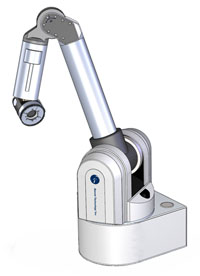
\includegraphics[height=4cm]{Img/set_up/wam.jpg}
\caption{Barrett WAM arm}\label{fig:wam_1}
\end{subfigure}
\begin{subfigure}[b]{0.45\textwidth}
\centering
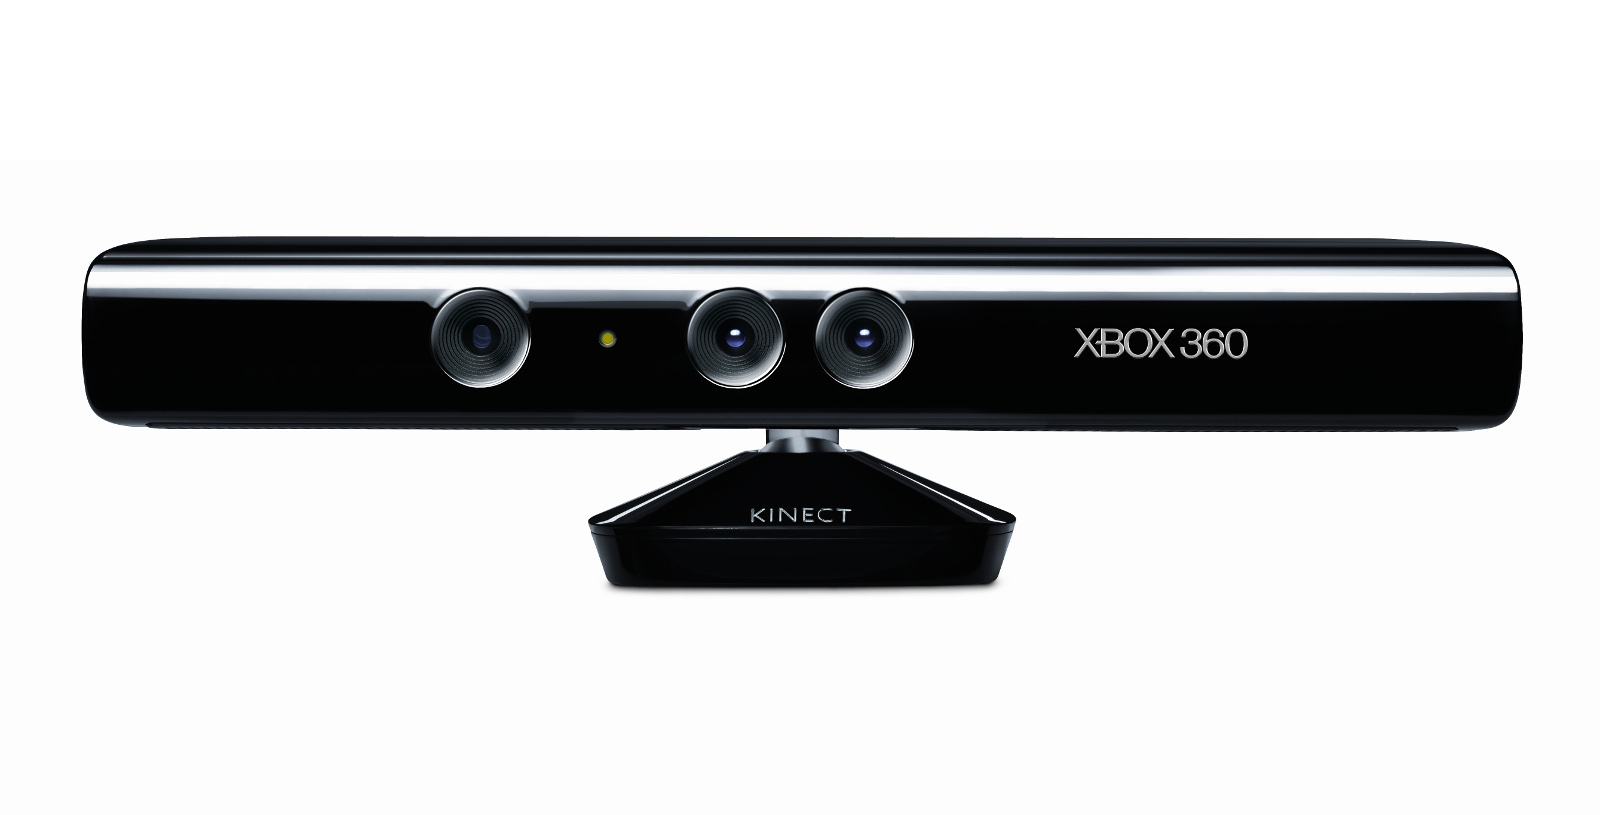
\includegraphics[width=5cm]{Img/set_up/Kinect.jpg}
\caption{Microsoft Kinect sensor}\label{fig:kinect}
\end{subfigure}
\caption{Robot and vision sensor.}
\end{figure}
%This robot is characterized by a low inertia of the end effector thanks to the kind of its actuators. 
The WAM is noteworthy because it does not use any gears for manipulating the joints, but cable drives, so there are no backlash problems and it is both fast and stiff. Cable drives permit low friction and ripple-free torque transmission from the actuator to the joints. 
To detect the objects a Kinect camera, a RGB-D sensor, is employed (\figref{fig:kinect}).

To manipulate the objects the robot has a gripper designed in the IRI institute and actuated by Dynamixel motors. Such a gripper is depicted in Figure \ref{fig:gripper_general} from several point of views. Its closing width\footnote{Distance between the fingers when the gripper is closed.} is $3$ centimetres while its opening width\footnote{Distance between the fingers when the gripper is open.} is of $7$ centimetres, therefore we are constrained to grasp objects with a width in the range $[3 \div 7]cm$.

\begin{figure}[tb]
\centering
\begin{subfigure}[b]{0.3\textwidth}
\centering
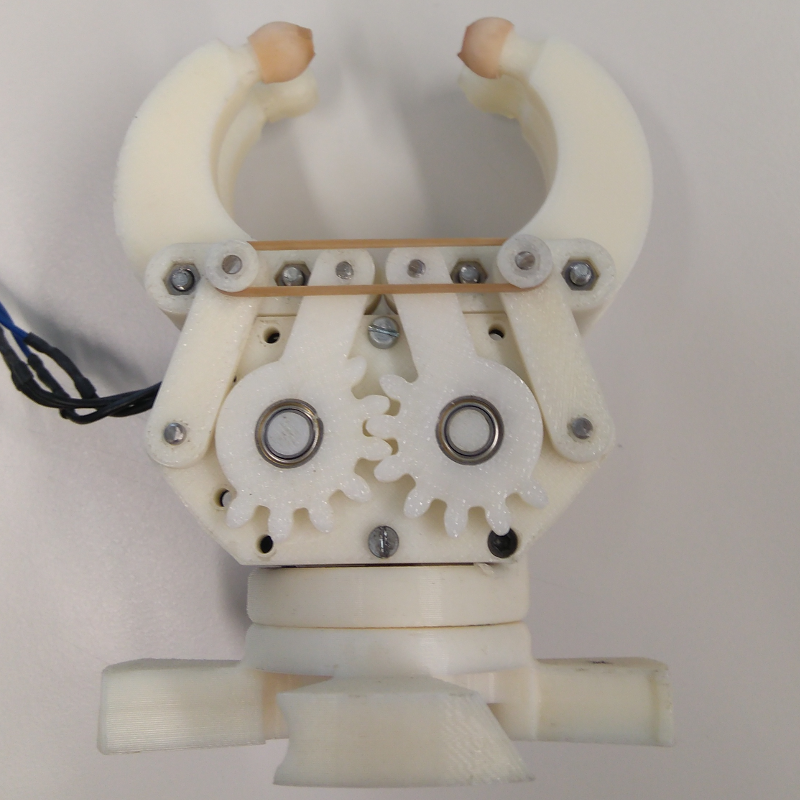
\includegraphics[height=3cm]{Img/set_up/gripper1.png}
%\caption{}
\end{subfigure}
\begin{subfigure}[b]{0.3\textwidth}
\centering
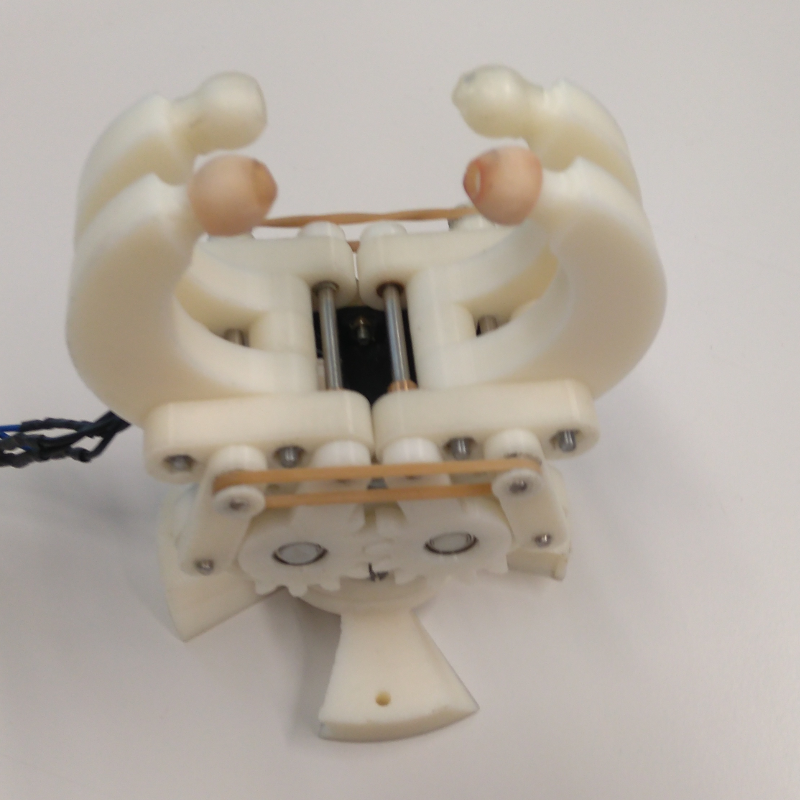
\includegraphics[height=3cm]{Img/set_up/gripper2.png}
%\caption{}
\end{subfigure}
\begin{subfigure}[b]{0.3\textwidth}
\centering
\includegraphics[width=3cm]{Img/set_up/gripper3.png}
%\caption{}
\end{subfigure}
\caption{Gripper used for the experiments}\label{fig:gripper_general}
\end{figure}

For the task planner, as the reader will see in Chapters \ref{ch:planning_system} and \ref{ch:implementation}, the model of the gripper will be an important resource 
in order to compute the predicates. 

The gripper will be modeled measuring some principal elements such as: finger's width and height, gripper's width, height and deep, closing and opening width. The modeling procedure is depicted in Figure \ref{fig:gripper_modelling}. The resulting model is a simple triangle mesh which includes all the important geometric information of the gripper.
\begin{figure}[tb]
\centering
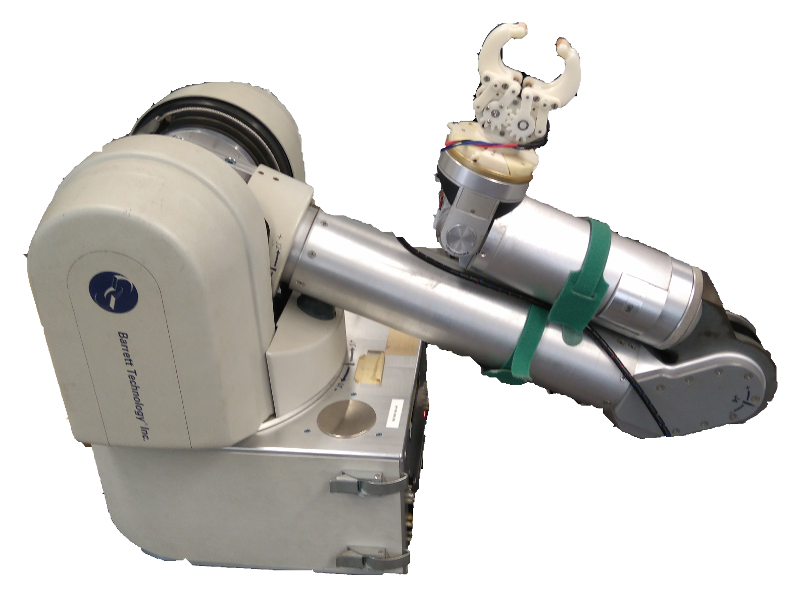
\includegraphics[width=5.0cm]{Img/set_up/wam_gripper2.png}
\caption{Gripper and WAM.}\label{fig:wam_gripper}
\end{figure}
Such a simple model allows the collision algorithm commented in Chapter \ref{ch:implementation} to check for collision in just a few milliseconds. 
A more detailed and complex model would have higher precision, but such a high accuracy is not needed, and it would slow down the algorithm. 
The gripper is mounted in the end effector of the robot as shown in Figure \ref{fig:wam_gripper}. 


\begin{figure}[tb]
\centering
\begin{subfigure}[t]{0.25\textwidth}
\centering
\stackunder[5pt]	{\includegraphics[height=3cm]{Img/set_up/gripper_modelling1.png}}{Elements measured}
\end{subfigure} 
\begin{subfigure}[t]{0.3\textwidth}
\centering
\stackunder[5pt]	{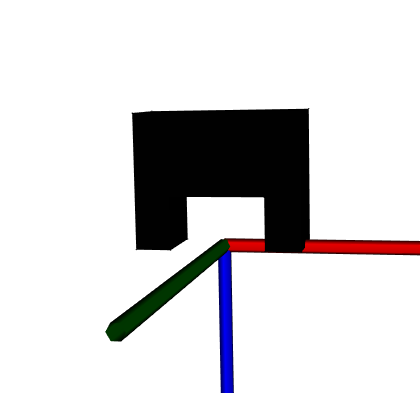
\includegraphics[height=3cm]{Img/set_up/gripper_open_model.png}}{Opened gripper mesh model}
\end{subfigure}
\hspace{1cm}
\begin{subfigure}[t]{0.3\textwidth}
\centering
\stackunder[5pt]	{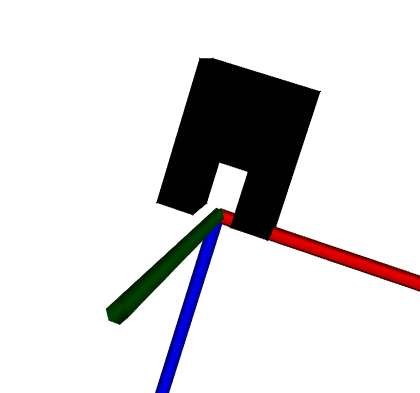
\includegraphics[height=3cm]{Img/set_up/gripper_closed_model.png}}{Closed gripper mesh model}
%\caption{}
\end{subfigure}
\caption{At the left the principal elements measured are highlighted for the opened gripper model. The gripper mesh model is here shown in the PCL visualizer. The \textcolor{red}{red}, \textcolor{green}{green} and \textcolor{blue}{blue} axis are respectively the x, y and z axis. }\label{fig:gripper_modelling}
\end{figure}

The scenario the robot is going to work in is composed of a table and the objects will lay on top of it. In Figure \ref{fig:setup_} the main elements of the set up are highlighted. The WAM arm's base is in a fixed position with respect the table and the Kinect camera is located on top of the table pointing down. The Kinect is calibrated and the fixed transformation between the Kinect's frames and the base frame of the robot is known, so all the points measured by the Kinect can be expressed in coordinates with respect the robot's base frame. Figure \ref{fig:example_scene} shows an example of a cluttered scene the robot is going to deal with, and Figure \ref{fig:kinect_view} shows the same scene as seen by the Kinect. %\DMcomment{Maybe say it in the opposite way: Figure X shows an example of a cluttered scene, and Fig. Y shows that same scene as seen from the Kinect camera.}
To avoid occlusions, we wait until the robot finishes to execute an action and moves away before taking new images. 

\begin{figure}[tb]
\centering
\begin{subfigure}[b]{0.4\textwidth}
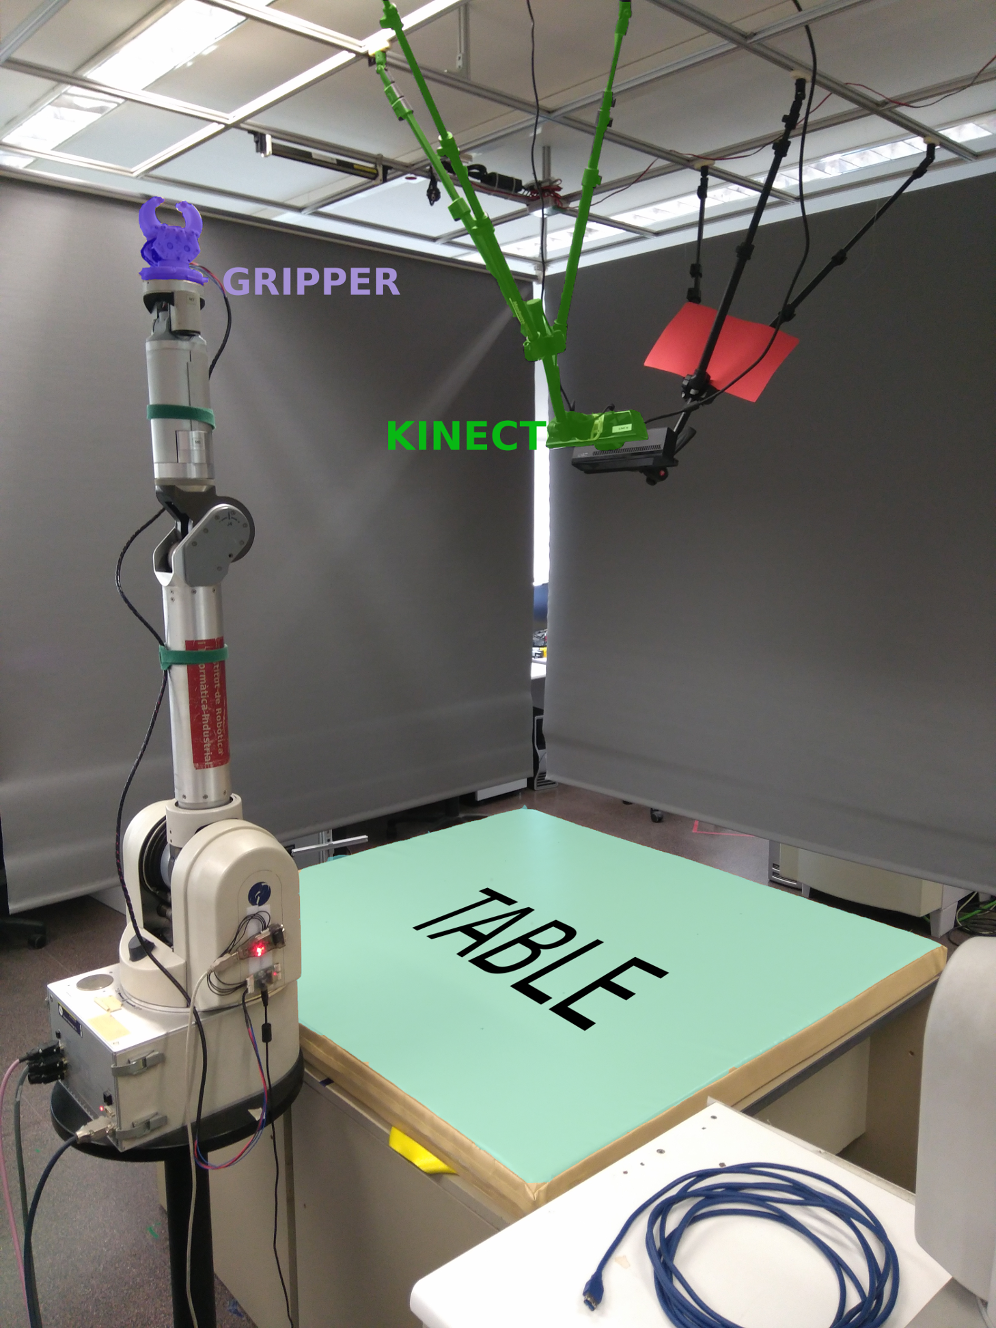
\includegraphics[height=8.5cm]{Img/set_up/set_up_nice2.png}
\caption{Principal elements of the experimental set up.}\label{fig:setup_}
\end{subfigure}
\qquad \qquad 
\begin{subfigure}[b]{0.4\textwidth}
\centering
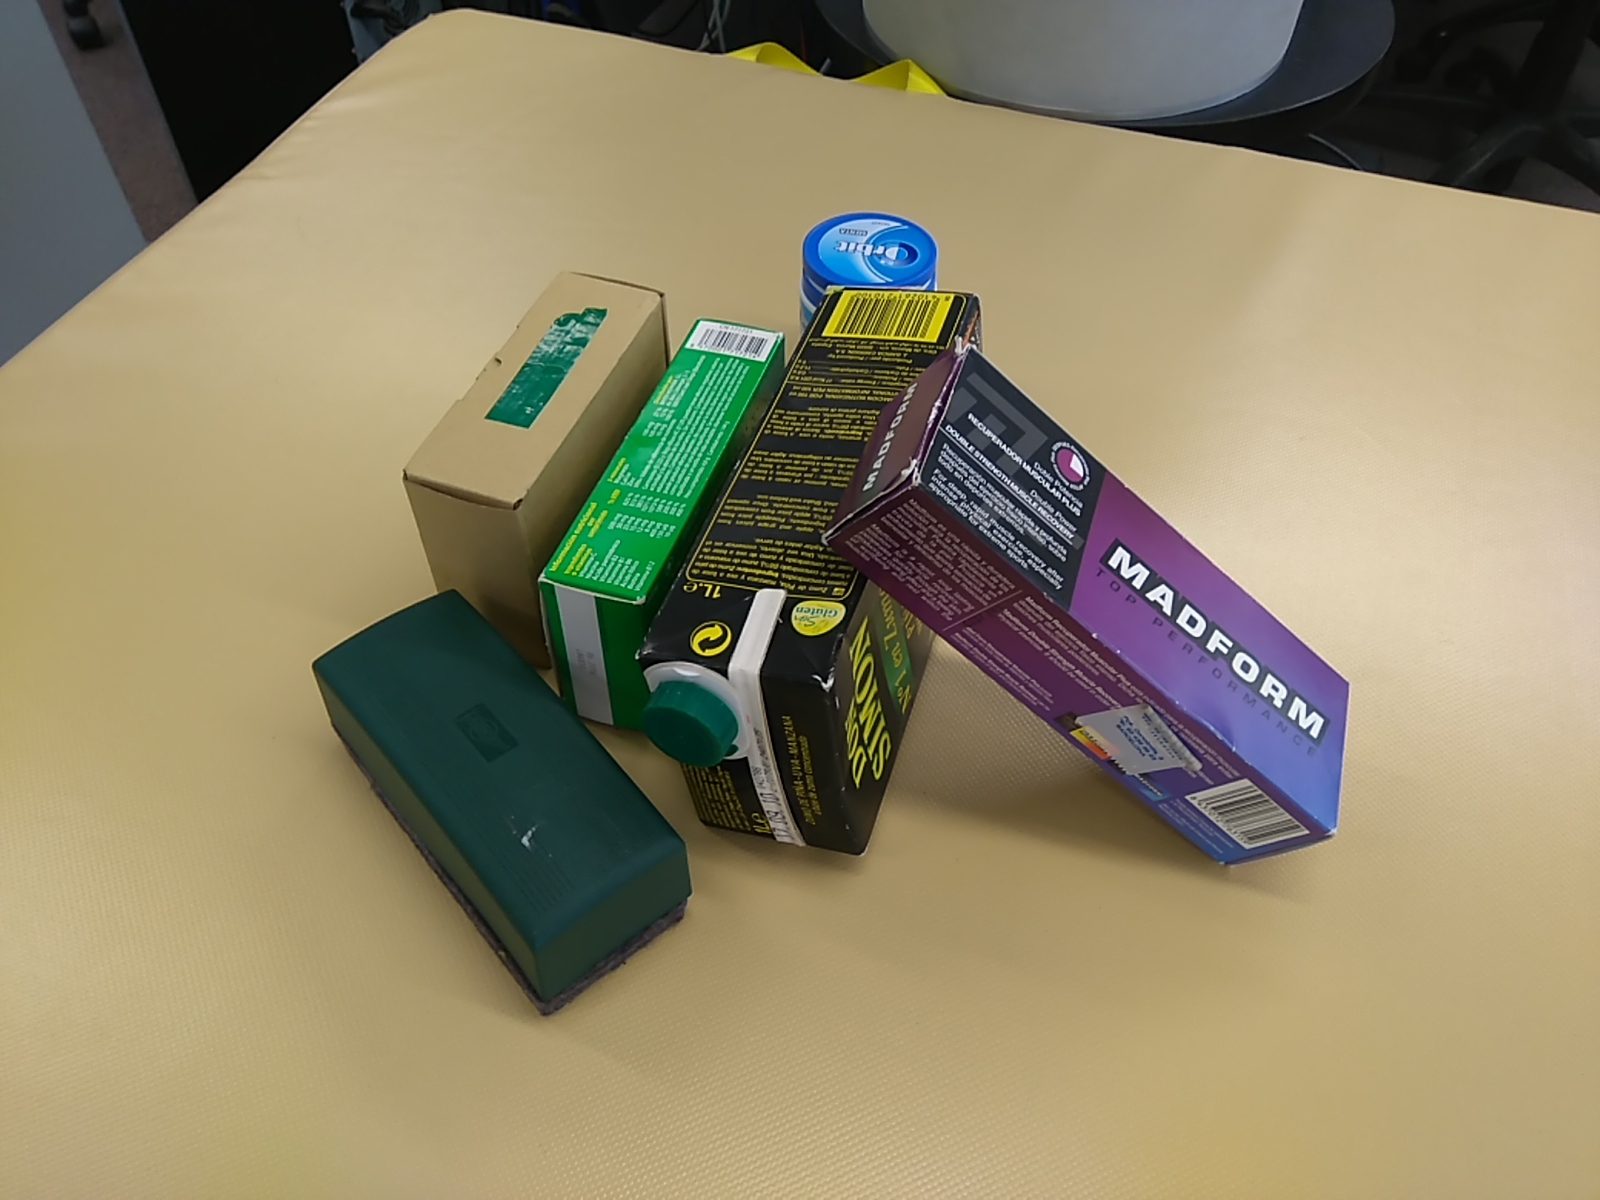
\includegraphics[height=4cm]{Img/set_up/examplesetup.jpg}
\caption{Example of a cluttered scene.}\label{fig:example_scene}
\vspace{2ex}
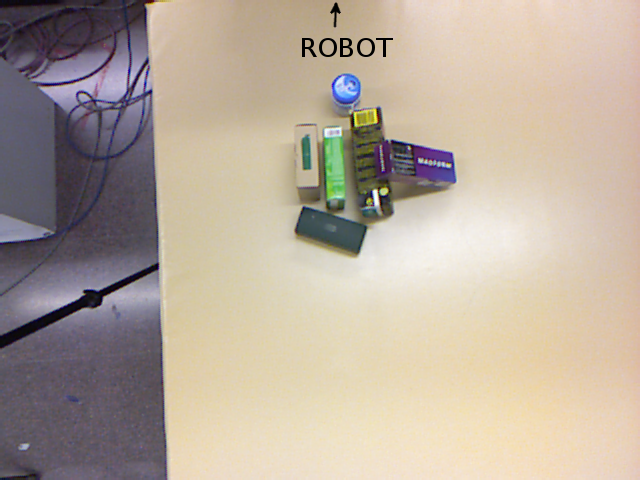
\includegraphics[height=4cm]{Img/set_up/view_kinect2.png}
\caption{Kinect's view.}\label{fig:kinect_view}
\end{subfigure}
\caption{Experimental set up with an example of a cluttered scene the robot is going to interact with.}
\label{fig:setup}
\end{figure}


%Concerning the example of Figure \ref{fig:example_scene} it can be appreciated that the manipulation needed in order to clean all the table with carefulness is quite complex. All the sequence of actions will be retrieved by the planner.



